\chapter{Association Matrix Learning}\label{sec:aml}

The TCM requires two association matrices, $\mtf$ and $\mft$, to be updated.
To translate this into neurons, an appropriate learning rule, the association matrix learning rule (AML), has to be derived.
The TCM gives the update of such an association matrix as
\begin{align}
    \mat M_{i+1} &= \mat M_i + \Delta \mat M_i \\
    \Delta \mat M_i &= \vc v_i \vc u_i\Tr
\end{align}
for adding an association from $\vc u_i$ to $\vc v_i$.
The association matrix after $n$ updates can be expressed as
\begin{equation}
    \mat M_n = \mat M_0 + \sum_{i=1}^{n} \Delta \mat M_i = \mat M_0 + \sum_{i=1}^n \vc v_i \vc u_i\Tr \text{.}
\end{equation}
This allows us to express the neural connection weights after learning $n$ associations as
\begin{equation}
    \weights = \menc \mat M_n \mdec = \menc \mat M_0 \mdec + \menc \sum_{i=1}^n \vc v_i \vc u_i\Tr \mdec
\end{equation}
where $\menc$ is the post-synaptic encoder matrix and $\mdec$ are the pre-synaptic decoders of the identity function.
This equation gives us some important information on how the learning of such association matrices can be implemented.
First, preexisting weights can be implemented as a transform on a normal neural connection that is kept constant.
Second, all the weight changes can be collapsed into decoder changes.
Thus, we need the AML to implement the decoder change given by
\begin{align}
    \tilde{\mdec}_{i+1} &= \tilde{\mdec}_i + \Delta \tilde{\mdec}_i \\
    \Delta \tilde{\mdec}_i &= \vc v_i \vc u_i\Tr \mdec
\end{align}
where $\tilde{\mdec}$ is the matrix of learned decoders.

To implement this within a neural network, the discrete equation has to be converted into continuous form:
\begin{equation}
    \od{\tilde{\mat D}}{t} = \eta \vc v(t) \vc u(t)\!\Tr \mat D \label{eqn:aml}
\end{equation}
with learning rate $\eta$.
Note that while in the discrete formulation all associations are added in with the same strength, in the continuous formulation, the associative strength depends on the learning rate and presentation time.
This equation can be directly implemented with the NEF and thus realized with spiking neurons.
That alone, however, does not ensure the biological plausibility, as any mathematical formulation of synaptic weight changes could be implemented with the NEF\@.
There are also multiple ways to implement the equation with the NEF that have different implications about a potential biological realization.
In the following, several of these possibilities are discussed.


\section{Explicit calculation of weight change}
Both the cue $\vc u(t)$ and target $\vc v(t)$ are available as neural signals.
That allows the implementation of the calculation of the outer product $\vc v(t) \vc u(t)\!\Tr$ in a set of neural ensembles.
The multiplication of each pair of scalars can be accurately implemented in spiking neurons as demonstrated by \textcite{gosmann2015-1}.
Those ensembles can then be connected up to modulate the synaptic strengths from the pre- to the post-populations (see \cref{fig:aml-explicit}) by forming the transpose of the outer product, applying a transform of $\mdec\Tr\!$, and transposing back.
\begin{figure}
    \centering
    \begin{tikzpicture}[nef]
        \graph[no placement] {
            u/$\vc u$ [ext, at={(0, 0)}],
            v/$\vc v$ [ext, at={(2, 0)}],
            uv/$\vc v \vc u\Tr$ [net, at={(1, -1)}],
            u -> uv, v -> uv,
            pre [ens, at={(-1, -3)}, minimum size=30] -- mod/"" [minimum size=0, inner sep=0, at={(1, -3)}] -> post [ens, at={(3, -3)}, minimum size=30],
            uv -> [modulatory, "$\mdec\Tr$" right] mod,
        };
    \end{tikzpicture}
    \caption{Explicit neural calculation of the AML weight change.}\label{fig:aml-explicit}
\end{figure}

It might be surprising that the change in the connection weights between the pre- and post-ensemble does not depend on their own activity, but is controlled externally.
While this is different from many other common learning rules, there is evidence of such heterosynaptic learning in the brain and specifically the hippocampus \parencite{huilme2014,rebola2017,uchida2012}.
Furthermore, this learning rule requires some preexisting structure and connection weights to calculate the signal for the weight modulation.
But as most NEF models do not give a developmental account of how such structures come about, I put this question aside and leave it at something that has to be answered in the future and concerns any type of NEF model, not just this learning rule.
However, there is one more aspect that can be criticized as being biologically implausible: the connections from the outer product calculation depend on the decoders of the pre-population.
It is not clear how the pre-population could transmit this information to this other place.

A similar problem of biological plausibility occurs in classical neural networks and deep learning with back propagation, where the weights for the transmission of the error signal need to be symmetric to the forward weights.
Recently, this concern of biological plausibility in deep learning has been slightly alleviated by the discovery that the weight symmetry is not strictly required.
It is possible for the network to adjust its forward weights to account for existing, non-symmetric backward weights, a process known as feedback alignment \parencite{lillicrap2016}.
Unfortunately, it is not clear whether this can be applied to the situation here.


\section{Explicit calculation of weight change without weight symmetry}
By reformulating $\vc v(t) \vc u(t)\!\Tr \mdec$ as $\vc v(t)[\mdec\Tr \vc u(t)]\Tr$ it is possible to implement the learning rule without the need for a connection to be based on decoders of a neural ensemble it is not related to.
Again there is a set of neural ensembles calculating an outer product (see \cref{fig:aml-explicit-no-sym}).
\begin{figure}
    \centering
    \begin{tikzpicture}[nef]
        \graph[no placement] {
            v/$\vc v$ [ext, at={(2, 0)}],
            uv/$\vc v (\mdec\Tr \vc u)\!\Tr$ [net, at={(1, -1)}],
            v -> uv,
            pre [ens, at={(-1, -3)}, minimum size=30] -- mod/"" [minimum size=0, inner sep=0, at={(1, -3)}] -> post [ens, at={(3, -3)}, minimum size=30],
            pre -> ["$\mdec\Tr$"] uv,
            uv -> [modulatory] mod,
            u/$\vc u$ [ext, at={(-3, -3)}] -> pre,
        };
    \end{tikzpicture}
    \caption{Explicit neural calculation of the AML weight change avoiding weight sharing.}\label{fig:aml-explicit-no-sym}
\end{figure}
But in contrast to the previous approach, if the pre-ensemble is also used as the cue input $\vc u(t)$, the transform $\mdec\Tr$ applied to $\vc u(t)$ is based on that ensemble's decoders decoding $\vc u(t)$.
The transform could even be rolled into the decoder matrix
\begin{equation}
    \mdec_{*} = \mdec\Tr \mdec \text{.}
\end{equation}
As we generally assume, in the context of the NEF, that there is some mechanism in place to establish the decoders to compute arbitrary given functions, this might already be considered a satisfactory answer to the biological plausibility.

However, it is not possible to state the function to obtain the decoders $\mdec_*$ because the function itself depends on the encoding by the neurons.
Moreover, $\mdec_*$ is a symmetric matrix, which is a constraint not respected by the normal decoder optimization process.
But in the context of the NEF, it can be assumed that the neural network can decode the identity function, i.e., there is a connection with decoders $\mdec$.
This can be used to learn a connection with decoders $\mdec_*$.

Given the vector of neural activities $\vc \act$ at time $t$, we have $\vc x = \mdec \vc \act$ and can state
\begin{equation}
    \vc x\Tr \vc x = \vc \act\Tr \mdec\Tr \mdec \vc\act \overset{!}{=} \vc\act\Tr\mdec_*\vc\act \text{.}
\end{equation}
This gives us an error expression as
\begin{equation}
    \err^2(\vc\act) = \left\lvert\vc x\Tr \vc x - \vc\act\Tr \mdec_* \vc\act\right\rvert^2 \overset{!}{=} 0
\end{equation}
with the gradient defined as
\begin{equation}
    \pd{\err^2(\vc\act)}{\mdec_*} = 2 \del{\vc\act\Tr \mdec_* \vc\act - \vc x\Tr \vc x} \del{\vc\act \vc\act\Tr} \text{.}
\end{equation}
The gradient can be used for a weight update rule
\begin{equation}
    \od{\mdec_*}{t} = -\eta_* \pd{\err^2(\vc\act)}{\mdec_*}
\end{equation}
in a (spiking) neural network to perform stochastic gradient descent.

To demonstrate that this learning rule allows the learning of the desired symmetric matrix, it was applied to a connection where the pre-synaptic ensemble was fed with a randomly varying vector signal.
The vector was generated from bandwidth limited Gaussian white noise (upper limit \SI{40}{\hertz}) for each component, normalized, and then multiplied by a bandwidth limited white noise scalar.
The learning rate was set to $\eta_* = \SI{1e-13}{\second^{-1}}$.
We can see that the Frobenius norm of the difference between the learned matrix $\mdec_*$ and the desired matrix $\mdec\Tr\mdec$ continuously decreases (\cref{fig:aml:grad-err}).
The decoded output for some dimensions quickly aligns with the target output (\cref{fig:aml:grad-decode}), but that does not happen for all dimensions.
This might be due to the random input not sufficiently covering the representational space.
\begin{figure}
    \centering
    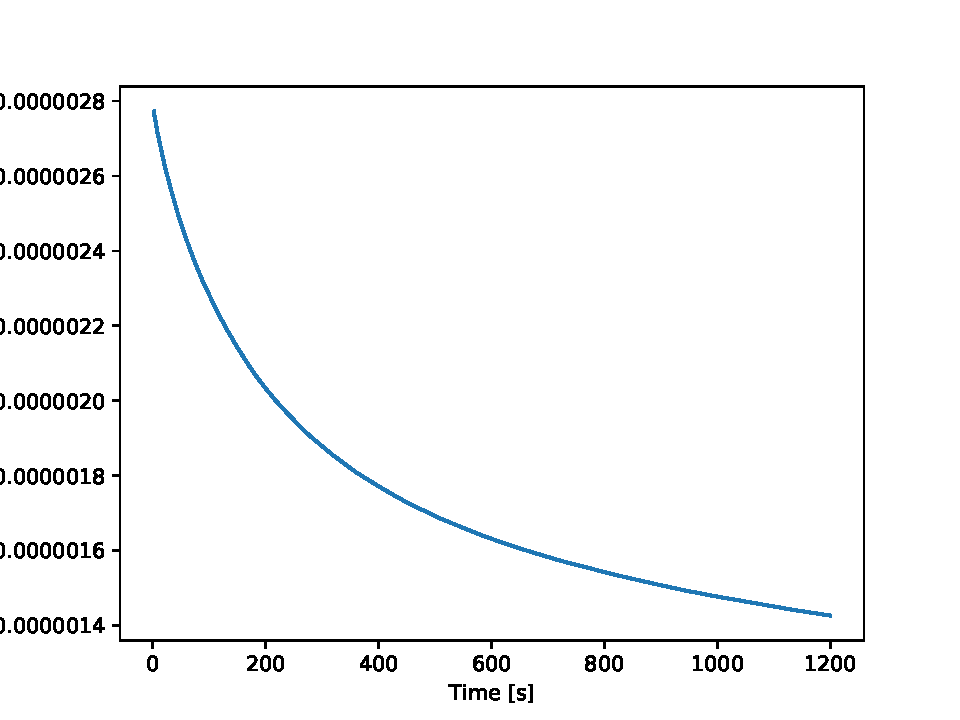
\includegraphics{figures/aml-grad-err}
    \caption{Error $\lVert \mdec\Tr\mdec - \mdec_*\rVert$.}\label{fig:aml:grad-err}
\end{figure}
\begin{figure}
    \centering
    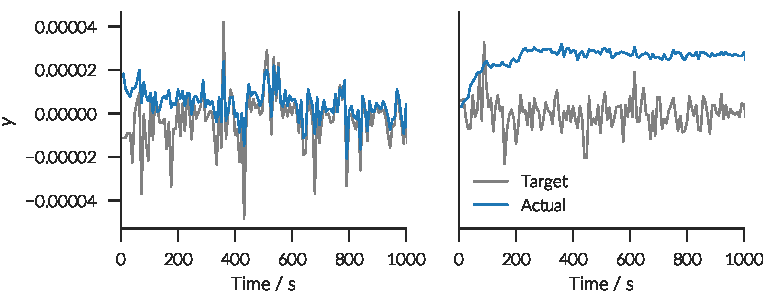
\includegraphics{figures/aml-decode}
    \caption[Example of two outputs decoded with the symmetric weights being learned.]{Example of two outputs decoded with the symmetric weights being learned. The output dimensions on the left quickly aligns with the target, while this does not happen (within the shown time frame) for the output dimension on the right.}\label{fig:aml:grad-decode}
\end{figure}

Again, the pure derivation of a learning rule does not ensure its biological plausibility.
Thus, let us consider the individual terms in the gradient.
The term $\vc\act\Tr \mdec_* \vc\act$ is using the current decoders to decode the ensemble's activity in no way different than usually done in the NEF where the existence of these standard decoders is generally assumed.
The decoded value is then correlated with the ensemble's activity.
The plausibility of this is somewhat unclear to the direct interaction of decoded values and neural activities, but to my knowledge there is no data excluding this possibility.
In particular, the decoded value and activities could be projected to another neural ensembles (see \cref{fig:aml-grad-desc}) that calculates the inner product.
The same, a projection to neural ensemble calculating the inner product, could happen with the decoded value $\vc x$.
Alternatively, $\vc x\Tr \vc x$ could directly be decoded (as a square of the individual components all projecting into the same dimension).
\Cref{fig:aml:neural-grad-err} shows the time course of the error when learning $\mdec_*$ with such a neural gradient computation.
The observed decrease demonstrates the basic viability of this approach, but the learning is slower and flattens out earlier due to the spiking noise.
\begin{figure}
    \centering
    \begin{tikzpicture}[nef]
        \graph[no placement] {
            pre [ens, at={(0, 0)}, minimum size=30] -- mod/"" [inner sep=0, minimum size=0, at={(2.5, 0)}] -> post [ens, at={(4, 0)}, minimum size=30],
            pre -> [bend left] act/"$\vc\act\Tr \mdec_* \vc\act$" [net, at={(0, 3)}],
            pre -> [bend right, "$\mdec_*$" xshift=-3mm] act,
            pre -> targetact/"$\vc x\Tr \vc x$" [net, at={(1.5, 1.5)}],
            act -> combine/"" [pnode, at={(3, 3)}],
            targetact -> ["$-1$"] combine,
            combine -> [modulatory, out=270, in=90] mod,
        };
    \end{tikzpicture}
    \caption{Neural computation of the error signal necessary for learning symmetric decoders with gradient descent.}\label{fig:aml-grad-desc}
\end{figure}
\begin{figure}
    \centering
    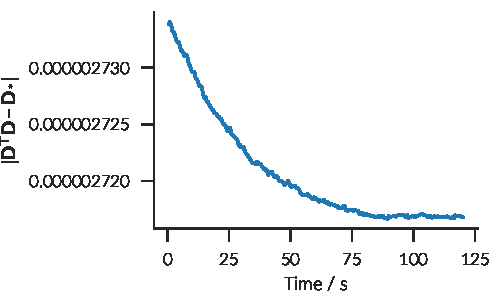
\includegraphics{figures/aml-neural-grad-err}
    \caption{Error $\lVert \mdec\Tr\mdec - \mdec_*\rVert$ with neural gradient calculation.}\label{fig:aml:neural-grad-err}
\end{figure}


The whole term $\vc\act\Tr \mdec_* \vc\act - \vc x\Tr \vc x$ is a scalar that influences all synapses.
This could be realized by a broadly acting neuro-modulator or by extensive connectivity of the neural ensembles calculating this error term.
Neither option is implausible.
This gradient term seems to play a role in weight normalization as it acts equally on all weights and the magnitude depends on the magnitude of the values of $\mdec_*$.
Also, without it all weight changes would always be negative.
Note that in many learning rules, normalization factors are often criticized as implausible for requiring knowledge of the whole weight matrix at the level of a single synapse.
This critique does not apply to this learning rule.
The decoding matrix is only used to decode from the activities which require only local knowledge of the weights.

Finally, the term $\vc\act \vc\act\Tr$ correlates neuron activities and appears somewhat Hebbian-like.
Hebbian learning is one of the best studied ways that biological systems learn.
In this form of learning pre- and post-synaptic neurons become connected when they fire in short succession.
In contrast to this usual account, here two pre-synaptic neurons connect to the same post-synaptic neuron if they fire together.
Again, the biological plausibility of this is somewhat uncertain, but cannot be outright rejected.


\section{Implicit error calculation}
The previous two implementations of the AML use minimal assumptions about the computational power of synapses.
All that is needed are additive weight changes proportional to some error signal.
However, it has been proposed that synapses might not simply transmit information, but also perform computations \parencites{abbott2004}[Ch.~5]{koch2004}.
In particular, \textcite{andreasstockel2018} showed that conductance-based synapses can be used in the NEF to compute nonlinear functions like multiplication.
That should allow us to roll the explicit outer product, required in the previous two approaches, into the synapses itself.
This requires considerably fewer neurons as no neural populations are required for each product.

In this thesis, I am using an implementation that corresponds to this implicit error calculation, but implements the required synaptic computation in pure math rather than implementing it with actual synaptic models.
This is mainly to reduce simulation times and is not meant as a statement that this is likely to correspond to the brain's implementation as there is not enough evidence to make such a strong claim.


\section{Normative interpretation}
While the AML cannot be outright rejected as biologically implausible, there are definitely some open questions concerning it.
Nevertheless, it should not be evaluated purely on this fact.
Many models in cognitive science, psychology, and computational neuroscience assume the encoding of associations in an outer product matrix \parencite[e.g.,][]{kajic2017,nowak2001,Brown2000}.
Ultimately, the validity of all those models depends on the possibility that the brain can learn such a matrix.
As such, the AML makes it explicit which operations have to be implemented to enable such learning.
If these turn out as either not being implemented in the brain or as not being implementable at all, it would follow that the brain has to use some other mechanism to represent associations.
Thus, the AML has merit as a normative theory, describing what the brain is ought to do, and directing research to open questions.

That being said, the AML does not make any assumption about the pre-synaptic neurons.
With such assumptions, some of the restrictions of the AML might be lessened.
For example, assuming orthogonal encoders, the decoder matrix $\mdec$ will be orthogonal too.
That in turn means that $\mdec_* = \mdec\Tr \mdec = \imat$ becomes the identity matrix which is independent of the exact decoders.
This simplifies connectivity and removes the need to learn the symmetric matrix $\mdec_*$ which alleviates some of the concerns of biological plausibility.

The dentate gyrus in the hippocampus is often assumed to perform pattern separation, which is a form of orthogonalization.
Hence, it might be possible that the hippocampus learns associations with a form of the AML where $\mdec_*$ ends up being the identity matrix and thus simplifies the learning rule itself.


\section{Properties of the AML}
So far the considerations about the AML were purely theoretical.
\Cref{fig:aml} demonstrates that an implementation of the AML can indeed learn associations in a spiking neural network.
Five different cue-target pairs were presented for one second each, before testing the recall with the same cues, but no target vectors.
The initially presented target vectors are almost perfectly recalled.
Note that no catastrophic forgetting occurred and each association was learned with a single presentation of the cue-target pair (one-shot learning).
Most other learning rules exhibit destructive interference between the items in this scenario.
As an example, \cref{fig:aml} also shows the same experiment using the Prescribed Error Sensitivity (PES) learning rule \parencite{bekolay2013}, which is commonly used in NEF models \parencite[e.g.,][]{komer2015,Rasmussen2017}.
Here all associations except for the last get destroyed.
It is still possible to learn associations with PES, but it requires the presentation of each item multiple times in interleaved fashion, i.e., one-shot learning cannot be done to learn associations in a reliable way.
\begin{figure}
    \centering
    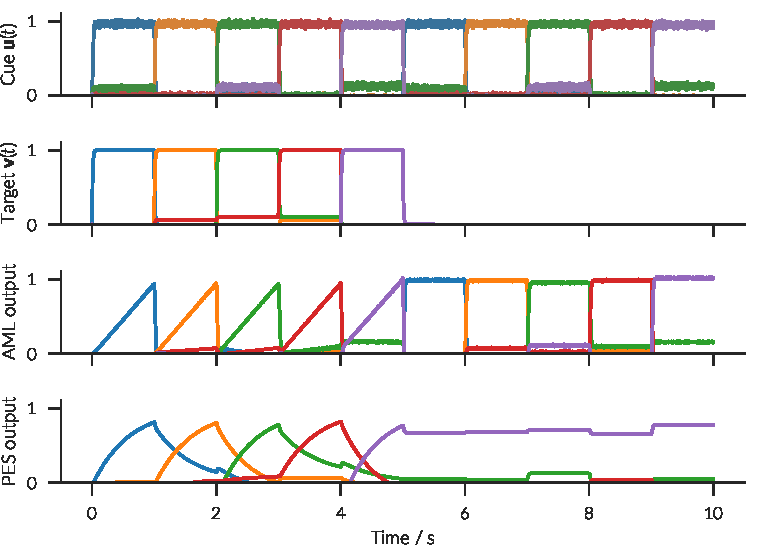
\includegraphics{figures/aml}
    \caption[Learning and recall testing of five cue-target pairs with the AML and PES.]{Learning and recall testing of five cue-target pairs with the AML and PES\@. Each colored trace is the dot product with one of the vectors used. The cue vectors $\vc u(t)$ and target vectors $\vc v(t)$ differ.}\label{fig:aml}
\end{figure}

This ability for one-shot learning with the AML is due to the $\mdec_*$ matrix, which accounts for the interference between neurons.
In fact, the AML and PES are the same except for that matrix.
The PES learning rule can be expressed as
\begin{equation}
    \od{\tilde{\mdec}}{t} = \eta \vc v(t) \vc\act_{\vc u}\Tr(t) \text{,}
\end{equation}
while the AML learning rule can be written as
\begin{equation}
    \od{\tilde{\mdec}}{t} = \eta \vc v(t) \vc u(t)\!\Tr \mdec = \eta \vc v(t) \vc\act_{\vc u}\Tr(t) \mdec\Tr \mdec
\end{equation}
which is the same, except for $\mdec_* = \mdec\Tr \mdec$.

The one-shot learning ability comes with some limitations, though.
The learning rule is restricted to learn transformations that can be expressed as outer product matrices, while learning rules like PES can learn arbitrary transformation matrices.
Moreover, the learning rule is essentially trying to learn a look-up table, mapping items to other items.
Thus, one should not expect the AML to generalize to unseen mappings.

This might be another reason, besides the stability-plasticity dilemma, why a two-stage memory system is needed.
The first stage would learn simple associations with the AML and only in the second step of consolidation with a different learning rule, commonalities get extracted for generalization.
This is consistent with data that shows that generalization improves with sleep.
For example, sleep improves transitive inference \parencite{stickgold2013-2} and gives insight into implicit rules \parencite{wagner2004}.
Experience replay in hippocampus might be responsible for the necessary interleaving of memory traces when using a learning rule that allows for more generalization, but exhibits destructive interference such as PES \parencite{mcclelland1995-1,kumaran2016}.
Overall, it is likely that AML only represents a first step in the association learning process and multiple learning rules are at play here.
That the brain uses no single general purpose learning rule, but combines different learning rules has been forcefully argued by \textcite{gallistel2009}.


\section{AML accounts for neural changes during association learning}\label{sec:aml-neural}
\Textcite{ison2015} reported that individual neurons in hippocampus (and parahippocampal cortex) change their firing rapidly to encode newly learned associations.
They recorded from the medial temporal lobe of \num{14} epilepsy patients that needed to undergo surgery.
They identified neurons that responded to specific visual stimuli of pictures of persons and landmarks and recorded the response to this \emph{preferred} (P) stimulus.
Then the participants learned associations between pairs of a person and a landmark.
Besides multiple tasks to assess the learning, the neuron responses to the different stimuli were recorded again after learning.

Pair-coding units could be identified that showed an elevated firing rate only to the preferred stimulus before learning (BL).
After learning (AL), those same units showed an elevated firing rate only to the preferred and associated non-preferred (NP) stimulus.
This can also be observed for associations learned with the AML\@.
\Cref{fig:aml-net} shows a NEF network that implements the learning of associations between persons and landmarks to reproduce the experiment by \textcite{ison2015}.
The connections weights from both pre-ensembles $\vc l$ and $\vc p$ are initialized with the identity transform.
To achieve firing rates closer to the recorded data, the maximum firing rates of the ensembles were sampled uniformly from \SIrange{10}{20}{\second^{-1}} (instead of \SIrange{200}{400}{\second^{-1}} used in the CUE model) and intercepts were sampled uniformly from \numrange{0.1}{1}.
The dimensionality of the ensembles and semantic pointers was set to \num{32}.
Furthermore, Gaussian white noise with a mean of \num{0.01} and standard deviation of \num{0.05}, low-pass filtered with a time-constant of \SI{0.1}{\second}, was injected into the neurons to account for neural background firing.
The recorded spikes were analyzed analogous to \textcite{ison2015}.
\begin{figure}
    \centering
    \begin{tikzpicture}[nef]
        \graph [no placement] {
            landmark [x=-2, y=0, ext] -> L/"$\vc l$" [x=0, y=0, ens] -- c1/"" [inner sep=0, minimum size=0, x=2, y=-0.5] -> post [x=4, y=-1, ens];
            person [x=-2, y=-2, ext] -> P/"$\vc p$" [x=0, y=-2, ens] -- c2/"" [inner sep=0, minimum size=0, x=2, y=-1.5] -> post;
            L -> err/"" [x=1, y=-1, pnode] -> [bend right, modulatory] c1;
            P -> err -> [bend left, modulatory] c2;
            post -> output/"" [x=6, y=-1, ext];
        };
    \end{tikzpicture}
    \caption[NEF network for associating two stimuli with the AML.]{NEF network for associating two stimuli (persons with landmarks here) with the AML.}\label{fig:aml-net}
\end{figure}

The main results obtained from the experimental and model data are shown in Figs.~\ref{fig:aml-spikes} and~\ref{fig:aml-population-response}.
\begin{figure}
    \centering
    \subcaptionbox{Experimental data}{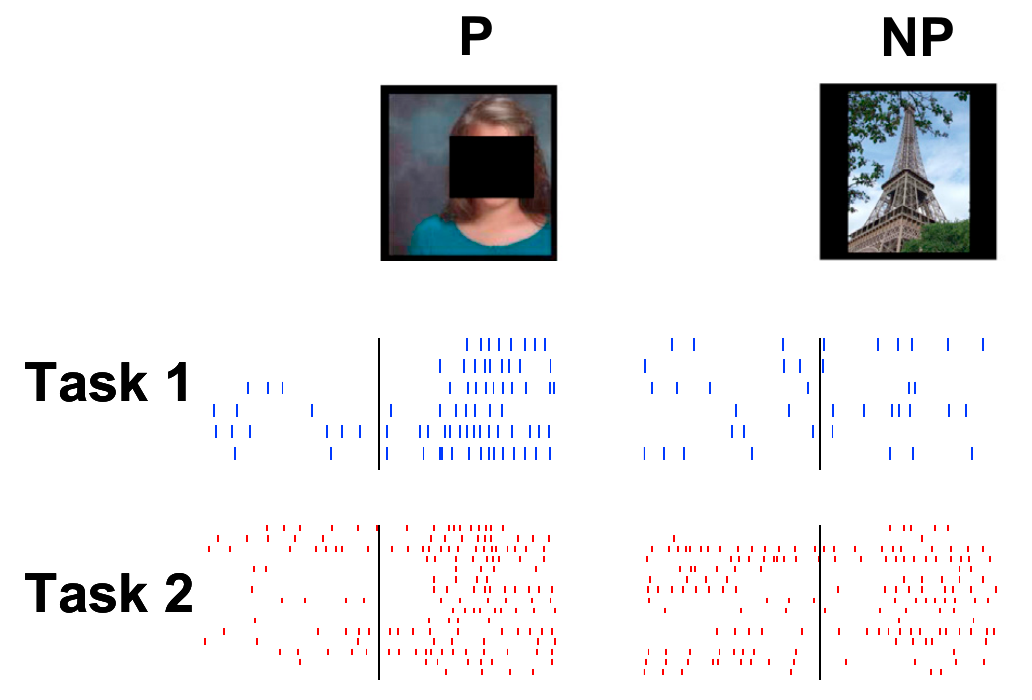
\includegraphics[width=9cm]{figures/ison2015-spikes}}

    \vspace*{0.34cm}
    \subcaptionbox{Model data}{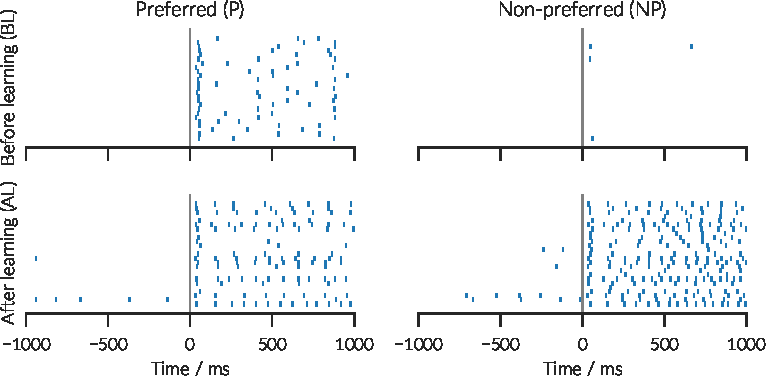
\includegraphics{figures/aml-spikes}}
    \caption[Change in spiking behaviour when learning associations.]{Change in spiking behaviour when learning associations. (a) Exemplary spikes recorded from human hippocampus for the preferred (P) and non-preferred (NP) stimulus. Task 1 (blue) is before, task 2 (red) after learning the P-NP association. The black line marks the stimulus onset. Figure adopted from \textcite{ison2015} under the Creative Commons Attribution 4.0 International license. (b) Spikes recorded from the NEF model learning the P-NP association with the AML\@.}\label{fig:aml-spikes}
\end{figure}
\begin{figure}
    \centering
    \subcaptionbox{Experimental data}{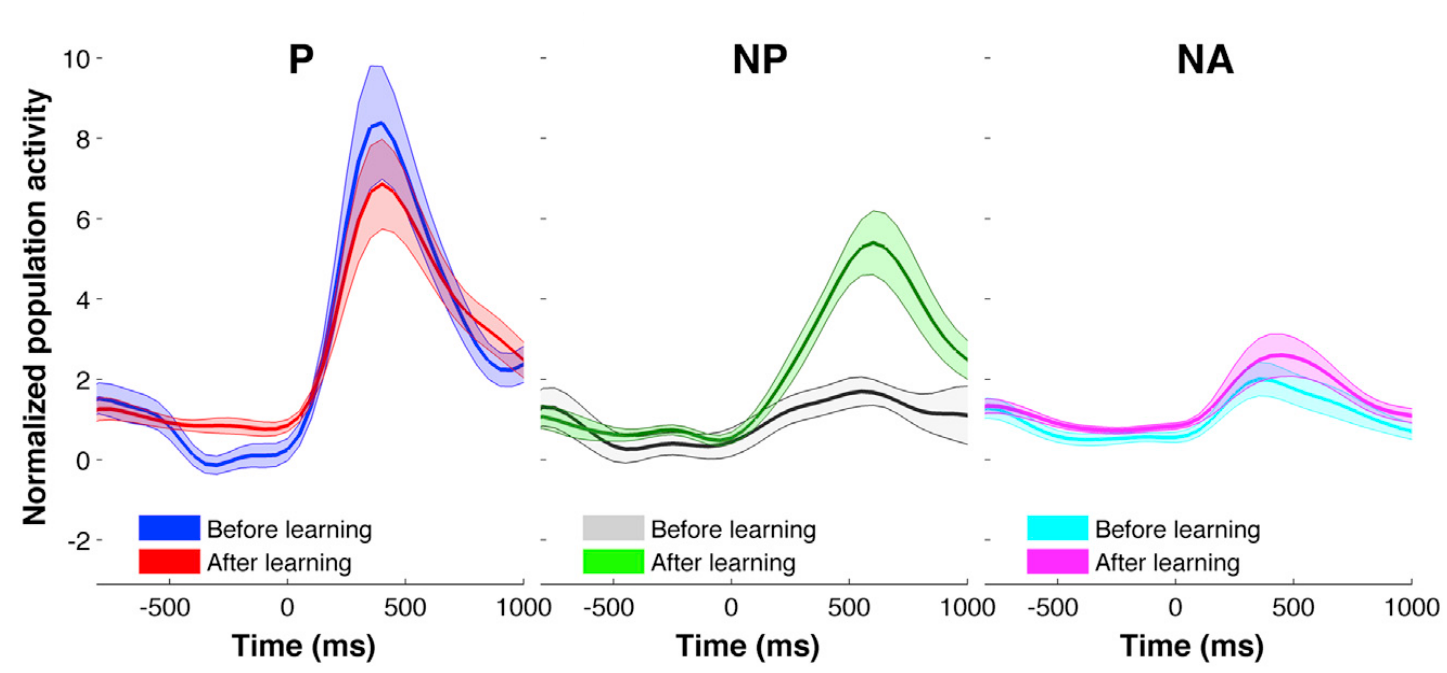
\includegraphics[width=12cm]{figures/ison2015-pop}}

    \vspace*{.75cm}
    \subcaptionbox{Model data}{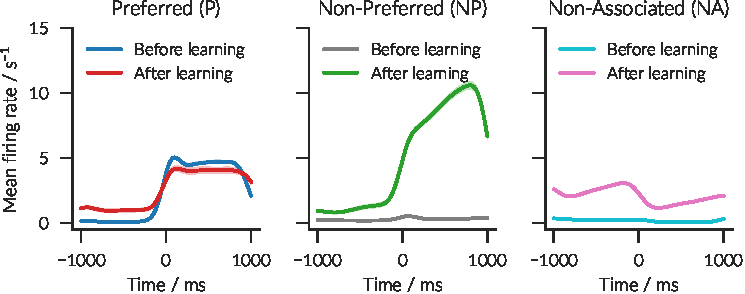
\includegraphics{figures/aml-population-response}}
    \caption[Population response for pair-coding units.]{Population response for pair-coding units to the preferred (P), non-preferred (NP), and non-associated (NA) stimuli before and after learning. Times are relative to stimulus onset. Shaded regions indicate the standard error of mean. (a) Normalized population activity from (a) experimental and (b) model data. Figure (a) adopted from \textcite{ison2015} under the Creative Commons Attribution 4.0 International license.}\label{fig:aml-population-response}
\end{figure}
Pairwise coding units, showing elevated firing in response to the preferred stimulus before learning and the non-preferred stimulus after learning without an increased response to any other stimuli, have been selected.
The normalized population activity in response to the preferred stimulus shows no or only a minimal change with learning in both the experimental and model data.
For the non-preferred stimulus the population activity increases slightly on stimulus onset which is more pronounced in the model data.
This might be explained by the model not including any visual processing that could delay and smooth out that response.
After learning, this population response is increased in both sets of data.
For non-associated stimuli the model shows a minimal decrease in the normalized population activity with learning, while the experimental data shows no significant change.
Overall, the model matches the main aspects of the experimental observations.
A better quantitative fit might be achievable with more careful parameter selection in the model.


\section{Weight normalization}
Note that the AML allows weights to grow without bound.
By introducing a factor of $1 - \vc v(t)\!\Tr \hat{\vc v}(t)$ this can be prevented where $\hat{\vc v}(t)$ is the retrieved, learned association.
But similar to other weight normalizations it introduces the need for each weight to have access to the global population activity and weights as $\hat{\vc v}(t) = \tilde{\mdec} \vc\act_{\vc u}(t)$.
Such global dependencies are often criticized for not being biologically plausible.
As such, I decided to take a slightly different approach with an equivalent effect.
Instead of including the dot product $\vc v(t)\!\Tr \hat{\vc v}(t)$ in the learning rule, it can be computed by another neural population and the thresholded result can be used to inhibit the population providing $\vc v$.
Once fully inhibited, $\vc\act_{\vc v}(t)$ will be all-zero and thus prevent further weight changes.
In the CUE model, the inhibition threshold is adjusted to follow $1 + \exp(-t)$ for learning the $\mtf$ matrix where $t$ is the time since the trial started.
This is intended to account for rehearsal effects that are not explicitly modelled and is analogous to the extended TCM model by \textcite{Sederberg2008}.
